%PART_3_CHAP_3_SEC_1
%WAIT a Review, ok
\section{Utilisabilité et UX}\label{Exp:L_UX}
    \subsection{Introduction}
        Pour réaliser cette étude, nous avons sélectionné deux questionnaires standardisés traitant de cette question: le \sht{SUS}~\citeA{pdf:SUS} et l' \sht{ATT}~\citeA{pdf:ATT}.
        Ces deux questionnaires sont complémentaires et permettent, d'un côté d'identifier d'éventuels problèmes de conception et de l'autre de rendre compte de la perception de l'utilisateur lors des activités.
        L’intérêt qu'ils soient standardisés est de pouvoir comparer les résultats.
    \paragraph{Méthode} 
        Le lien de ces questionnaires (à compléter en ligne) a été diffusé aux enseignants participant au dispositif Poppy-Éducation, qui l'ont ensuite transmis à leurs élèves.
        Nous avons collecté $88$ réponses: $20$ enseignants de $47$ ans en moyenne (écart type~$S=14,26$) et $68$ élèves ($\hat{a}ge=16$;~$S=2,44$),  $37$ sont issus de section ISN, $12$ de ICN, et $18$ du collège ($17$ de 3ème et $1$ de 4ème).
        Il ont tous pratiqué des activités durant l'année scolaire 2016 -- 2017 et ont répondu aux questionnaires à la fin de cette même année.
        Ces activités ont pu être plus ou moins longues, plus ou moins répétées;
        pour déterminer ces paramètres un questionnaire de renseignements additionnels était intégré après les questionnaires d'utilisabilité, permettant de dégager 29~critères de discrimination visibles sur la figure~\ref{fig:sus_val_moy} en page~\pageref{fig:sus_val_moy}.
        Nous avons également synthétisé certains de ces critères pour former des groupes:
        \textit{néophyte}, n'a pas utilisé d'autres kits et a pratiqué moins de 6~heures d'activités avec le kit ErgoJr;
        \textit{novice}, n'a pas utilisé d'autres kits et a pratiqué entre 6 et 25~heures d'activités avec le kit ErgoJr;
        \textit{expert}, a utilisé d'autres kits et a pratiqué plus de 25~heures d'activités avec le kit ErgoJr;
        cependant, ces groupes n'ont pas permis d'établir de distinction significative.
        En revanche, d'autres résultats peuvent être observés, en voici les principaux.
    \subsection{SUS}
        Nous pouvons observer sur la figure~\ref{fig:sus_chemin} que la moyenne générale (axe noir en gras) est positive sur l'ensemble des affirmations hormis la première, cela est peut-être induit par l'environnement scolaire proposant des plannings stricts et de nombreux modules à explorer.
        Les affirmations 4 et 8 offrent la plus grande variabilité suivant les modalités, l'affirmation 8 s'étale du \cro{non} à \cro{absolument non} montrant une bonne acceptance.
        L'affirmation 4 allant de \cro{non} à \cro{sans avis} associée aux affirmations 7, 3 et 10 (variant légèrement moins), évoquent les questions de prise en main et de capacité d'auto-formation, point que nous souhaitions optimiser.
        Ici cette variabilité semble montrer que notre action a eu un impact mais pas sur l'ensemble de la population.
        \begin{figure}[!h]
            \centering
            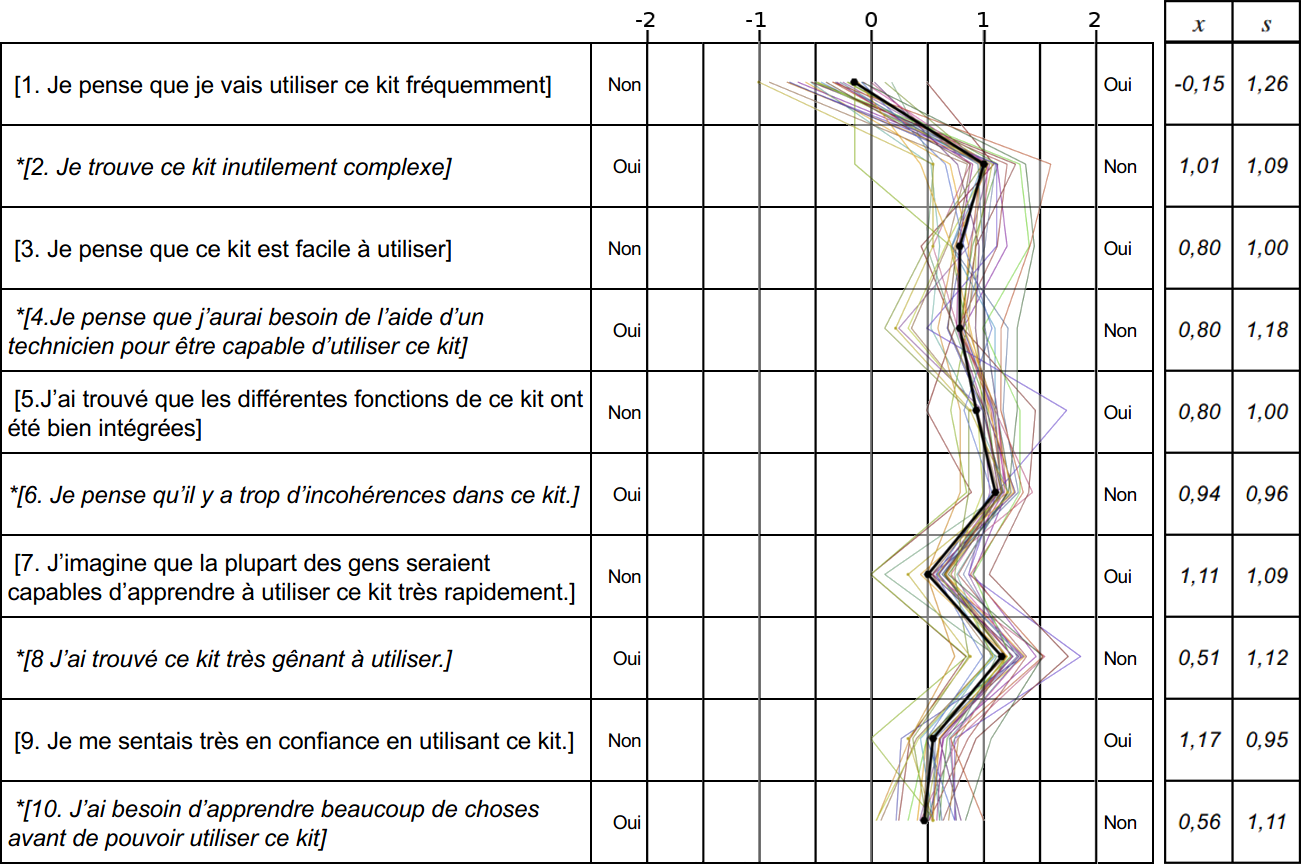
\includegraphics[width=0.9\linewidth]{Figures/Desprez_didapro-sus_chemin.png}
            \caption{Résultats SUS~\citeB{desprez2018poppy}}\label{fig:sus_chemin}
        \end{figure}
        La rétrospective de 2013 du \sht{SUS}~\citeB{brooke2013sus} nous apprend que le score moyen obtenu par des dispositifs au \sht{SUS} est de $68/100$ soit $0,72$ sur l'intervalle $[-2;2]$.
        Dans notre étude, la moyenne générale a atteint $0,72$: $0,57$ pour les enseignants et $0,77$ pour les élèves.
        Lorsque nous observons les résultats avec plus de détails, nous pouvons nous apercevoir (\textit{cf} Figure~\ref{fig:sus_val_moy}) que certains usages font varier significativement le score du \sht{SUS} de la moyenne ($Test\ de\ Student\ bilat\acute{e}ral\;\ \alpha=0,05\;\ ddl=9\;\ variable\ de\ r\acute{e}f\acute{e}rence=modalit\acute{e}\ \acute{E}l\grave{e}ves$), notamment:
        un temps d'utilisation inférieur à 2~heures ($p=0,0238$) ou une longue période entre la dernière utilisation du kit et le passage du questionnaire ($p=0,0007$) qui l'impacte négativement;
        l'utilisation du livret pédagogique ($p=0,0004$) qui l'impacte positivement;
        le choix du langage de programmation (\sht{snap} $p=0,0017$; python $p=0,0103$; autre $p=0,0019$) ayant un impact relatif au choix effectué:
        positif pour \sht{snap}, négatif pour python ou les autres langages (non natifs).\par%
        D'autre part, il est également intéressant d'observer les critères ne faisant pas varier significativement le score du \sht{SUS} comme l'utilisation d'autres kits ($p=0,3357$) ou non ($p=0,1683$);
        la construction du robot ($p=0,1029$) ou non ($p=0,2996$);
        ou encore la distinction entre \textit{Enseignants/Élèves} ($p=0,1687$) qui étaient des critères attendus comme discriminants.
        Cependant, concernant cette dernière, le faible effectif côté enseignants ($N=20$) peut expliquer l'absence de différence significative (\textit{cf 4.Limites \& perspectives}).
        Enfin, nous n'observons pas de distinction \textit{Homme/Femme} ($p=0,3740$), comme il est courant de trouver dans d'autres disciplines.
        \begin{figure}[!h]
            \centering
            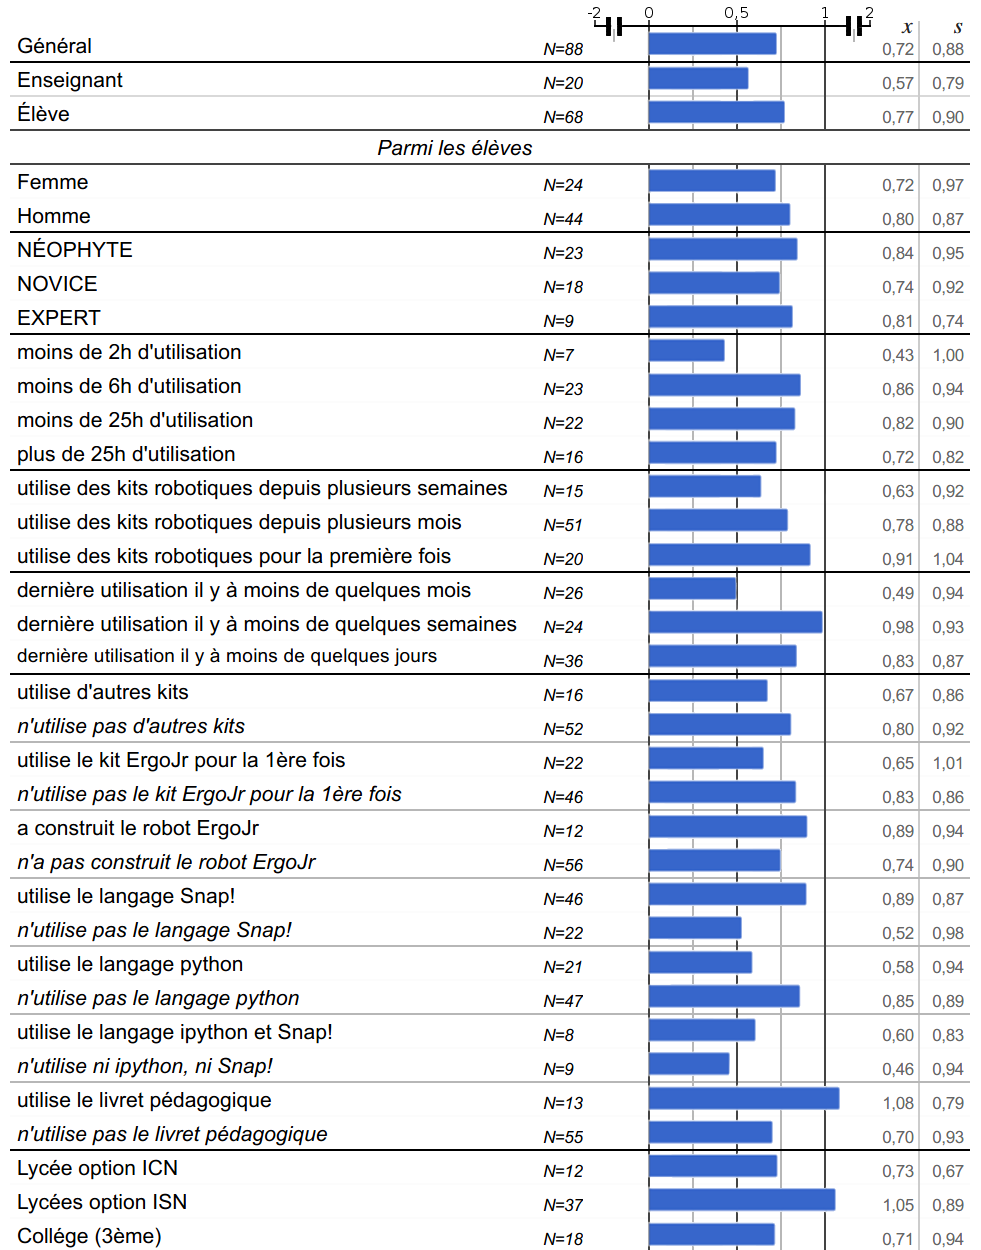
\includegraphics[width=0.9\linewidth]{Figures/Desprez_didapro-sus_val_moy.png}
            \caption{Résultats SUS, valeurs par groupes}\label{fig:sus_val_moy}
        \end{figure}
    \subsection{AttrackDiff}
        Nous pouvons observer sur la figure~\ref{fig:attrakdiff_chemin} le résultat pour nos 29 modalités pour les 28 paires de mots, ici ordonnées par catégorie.
        Sur la figure~\ref{fig:attrakdiff_chemin} nous pouvons voir qu'une majorité de réponses sont positives, et que plusieurs paires de mots semblent se distinguer, notamment:
        l'évaluation de \textit{Technique~/~Humain} en moyenne à $\overline{x}=-0,70$~($S= 1,38$) et l'évaluation de \textit{Amateur~/~Professionnel} à $\overline{x}=-0,15$~($S=1,45$) quand l'évaluation générale se situe à $\overline{x}=1,20$~($S=0,61$).
        Dans une moindre mesure nous observons la même distinction au niveau de \textit{Prévisible~/~Imprévisible} $\overline{x}=0,36$~($S=1,31$) qui peut s'expliquer par la mise en avant dans les activités de la démarche d'apprentissage par essai-erreur.
        De la même façon on observe que les termes \textit{Original - Créatif - Plaisant} obtiennent une meilleure évaluation que la moyenne, respectivement: $\overline{x}= 1,73; 1,75; 1,88$~($S= 1,24; 1,14; 1,15$).
        \begin{figure}[!h]
            \centering
            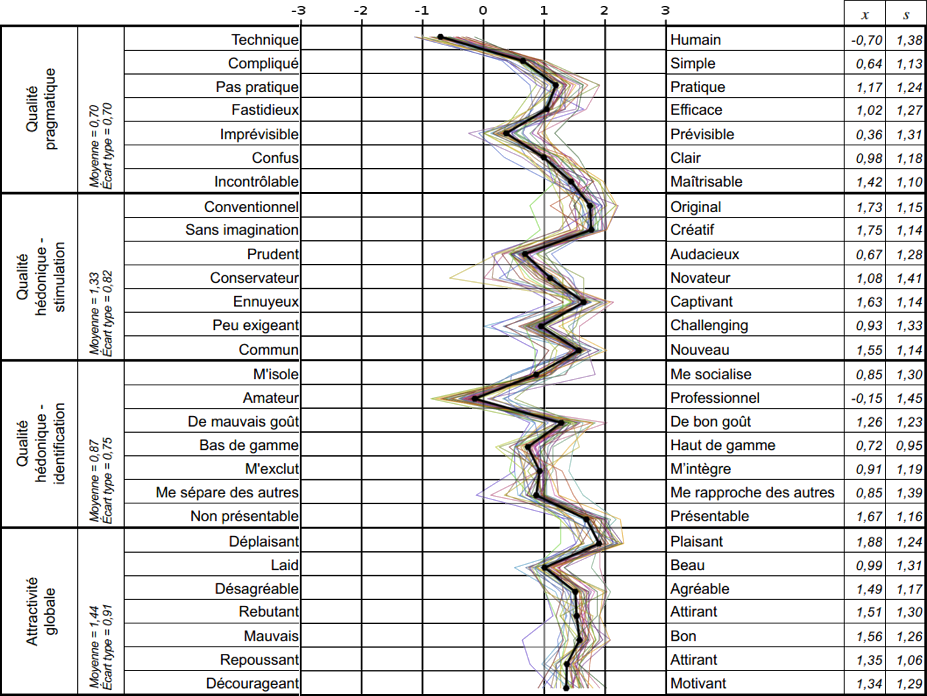
\includegraphics[width=0.9\linewidth]{Figures/Desprez_didapro-attrakdiff_chemin.png}
            \caption{Résultats \textit{AttrakDiff}~\citeB{desprez2018poppy}}\label{fig:attrakdiff_chemin}
        \end{figure}\par%
        Au niveau des 4 échelles, nous observons que l'aspect stimulation $\overline{x}=1,33$~($S=0,70$) et l'attractivité globale $\overline{x}=1,44$~($S=0,91$) obtiennent de meilleurs résultats que l'aspect identification $\overline{x}=0,87$~($S=0,75$) et pragmatique $\overline{x}=0,70$~($S=0,70$).
        La moyenne de ces différentes échelles donne un score global de $1,087$~($S=0,58$) pour l'ensemble de l'échantillon ($N=88$); de $1,057$~($S=0,58$) pour les enseignants ($N=20$); et de $1,182$~($S=0,61$) pour les élèves ($N=68$).
        Mais une représentation à deux dimensions nous permettra d'appréhender les résultats de manière plus efficiente.
        Ainsi nous pouvons observer, notamment sur la figure~\ref{fig:attrakdiff_point}, que la répartition globale est plutôt bien localisée:
        la moyenne générale se situe à $\overline{x}=1,07$~($S=0,64$) qui correspond à la valeur moyenne obtenue aux échelles \gui{Qualité~Pragmatique} et \gui{Attractivité~Globale}; et $\overline{y}=1,09$~($S=0,53$) qui correspond à la valeur moyenne obtenue aux échelles \gui{Qualité~Hédonique~Stimulation} et \gui{Identité}.
        En regardant par le prisme de nos 29 modalités, Nous observons que le nuage de points est plutôt homogène, mais certaines modalités (présentées sur la figure~\ref{fig:attrakdiff_point}) obtiennent des valeurs plus extrêmes par rapport à notre échantillon de base.
        \begin{figure}[!h]
            \centering
            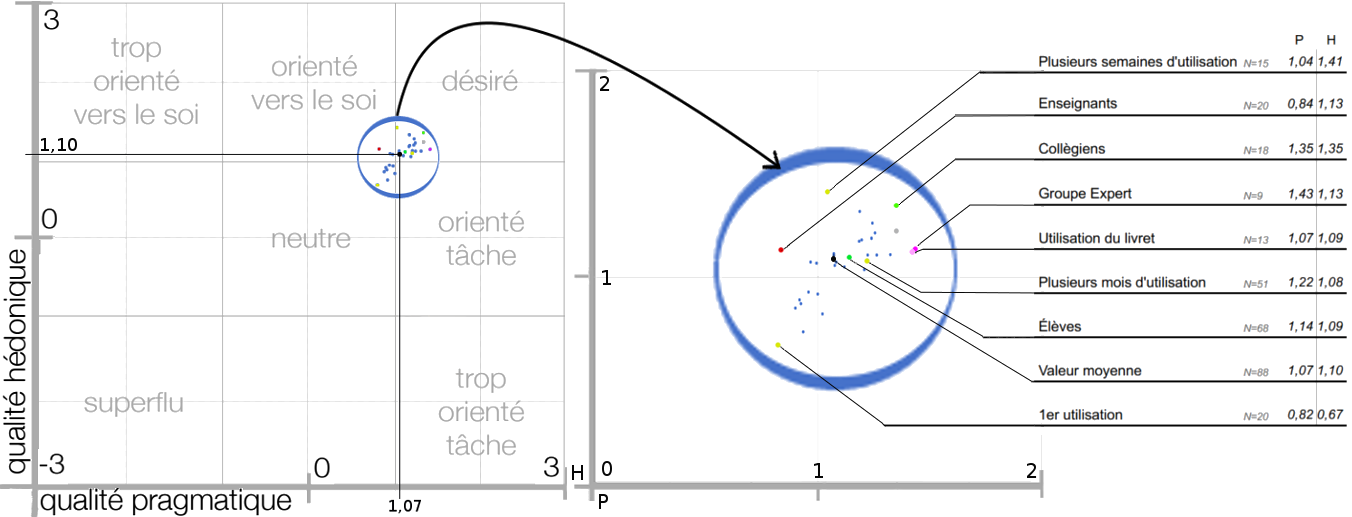
\includegraphics[width=0.9\linewidth]{Figures/Desprez_didapro-attrakdiff_point.png}
            \caption{Résultats \textit{AttrakDiff}, réduits à deux dimensions.}\label{fig:attrakdiff_point}
        \end{figure}\par%
        Tout d'abord nous pouvons observer que le groupe d'enseignants s'écarte significativement ($p=0,0564$, $ddl=28$) du groupe des élèves  ($Test\ de\ Student\ bilat\acute{e}ral\;\ \alpha=0,05\;\ ref\ var=\acute{E}l\grave{e}ves$), évaluant globalement la plateforme comme plus \gui{orientée~vers~le~soi} mais principalement causé par un score plus faible sur l'axe $x$ noté $P$ \gui{qualité pragmatique} ($p=0,00002$, $ddl=14$) (sur l'axe $y$ noté $H$ \gui{qualité hédonique} $p=0.7359$, $ddl=14$).
        Ceci peut être induit par la stratégie de conception qui plaçait les besoins \tiret{et~envies} de l'utilisateur au centre du développement.
        De plus l'enseignant adaptant le dispositif aux objectifs théoriques et pratiques qu'il s'est fixé, il semble cohérent que le score sur l'échelle pragmatique soit plus élevé chez les élèves, manipulant \textit{in~fine} le dispositif modifié par l'enseignant pour les besoins de la tâche ou du TP.
        Ensuite nous pouvons remarquer que le temps total d'utilisation de la plateforme modifie les résultats.
        Ainsi, manipuler le kit pour la première fois provoque une moyenne des réponses significativement plus neutre ($p=0,0000$), tandis que nous observons, pour le groupe l'ayant utilisé pendant plusieurs semaines, des valeurs significativement plus positives ($p=0,0004$) sur $H$;
        le groupe pratiquant depuis plusieurs mois est lui beaucoup plus proche de la la moyenne mais reste significativement différent sur $P$ ($p=0,0006$) et donc plus \gui{orienté vers la tâche}.
        De plus cette proximité avec la moyenne pourrait s'expliquer par l'effectif important de cette sous-catégorie d'élèves.
        Un autre fait remarquable se situe au niveau de la modalité \gui{utilise le livret pédagogique fourni} et le groupe \gui{Expert} qui obtiennent une évaluation similaire sur les deux échelles ($p=0,9469$) et qui est significativement différente de la moyenne sur $H$ et $P$ pour la modalité \gui{livret} ($p=0,0011$) mais uniquement sur $P$ ($p=0,0039$) pour les \gui{experts}.
        Enfin nous observons que le groupe des collégiens possède la meilleure évaluation globale, même si, individuellement ces moyennes sur les différentes échelles ne correspondent pas systématiquement à la valeur maximale.
    \subsection{Dans d'autres contextes}\label{Exp:vs_thymio}
        \paragraph{Introduction}
            Dans un second temps, il est intéressant d'observer et de mesurer l'utilisabilité du kit ErgoJr face à d'autres kits pédagogiques et surtout dans d'autres contextes. À noter qu'avec l'entrée de l'informatique dans le tronc commun des lycéens~\citeS{sec:programme-officiel} le besoin d'enseignant formé à cette matière pluridisciplinaire croit plus rapidement que annoncé. Ainsi, l'offre de formation \tiret{y compris en robotique} croit également, rendant l'étude de ce contexte pertinent. De plus, étant donné que l'élève représente une cible secondaire accessible uniquement via son enseignant~\citeS{sec:user_cible}, il semblait donc particulièrement intéressant d'éprouver notre kit dans un contexte de formation professionnelle.
        \paragraph{Méthode}
            Deux sessions de formation en robotique ont été organisées. Chacune dispensée sur une journée de 6~heures à des groupes de 16 adultes engagés dans une formation de deux semaines sur le numérique. Cette journée de robotique se divisait en deux: la matinée consacrée au robot Thymio, l'après-midi consacrée au robot Poppy ErgoJr. Les participants étaient invités à constituer librement des groupes de deux personnes pour l'ensemble des activités de la journée.
            Chaque demi-journée se clôturait par la passation individuelle de deux questionnaires validés: le \sht{SUS} et l' \sht{ATT}, rendant compte respectivement de l'utilisabilité et de l'expérience utilisateur.
            Aucune donnée personnelle sur les participants n'a été recueillie, et un total de 29 réponses complètes ont été collectées.
            \subparagraph{Déroulement des activités}
                Pour cette journée, il a été demandé au formateur de définir un robot comme étant une composition de capteurs et d'effecteurs associés à un micro-contrôleur contenant sa programmation et que de son interaction avec l'environnement émergeait un comportement. Le second objectif était d'introduire des notions élémentaires de la programmation, à savoir, les conditions et les boucles.
                %thymio
                Les activités de la matinée étaient constituées des missions 1, 2, 3, 4 puis la mission 10 extraite du parcours \textit{IniRobot}~\citeB{roy2016inirobot}. Les deux premières se focalisent sur l'observation et la découverte du robot face à 4 comportements pré-programmés. Les documents fournis viennent les guider vers un formalisme \textit{Si~\dots Alors~\dots} (\eg en mode jaune, si je mets un obstacle à gauche alors Thymio tourne à droite). À partir de la mission 3,\sht{vpl} est introduit. Ce langage de programmation événementiel et entièrement visuel propose de manipuler 2 types de cartes (\eg cartes capteurs et effecteurs) à associer via le formalisme \textit{Si~\dots Alors~\dots} sur la zone de script centrale~\citeT{tab:langue}. La mission 10 était consacrée à la réalisation d'un parcours d'obstacles présentés comme un défi où les participants sont invités à coder un programme similaire au comportement explorateur (mode jaune) observé durant les missions précédentes.
                %ergo
                Les activités de l'après-midi étaient constituées de deux activités de découverte pour le robot ErgoJr: l'activité \textit{caméléon}~\citeA{pdf:act_cameleon}focalisée sur les capteurs et l'activité \textit{chamboule~tout}~\citeA{pdf:act_chamboul} focalisée sur les effecteurs.
                La première partie de l'activité \textit{caméléon} est destinée à la prise en main de l'interface \sht{snap}~\citeT{tab:langue} et des principes de la programmation visuelle par bloc~\citeB{harvey2012snap}: mode d'interaction par cliquer/déposer, activation de plusieurs séquences d'instructions en parallèles, typage des blocs, \etc. La seconde partie propose un défi où l'objectif est de faire varier la couleur des leds présentes sur le robot en fonction d'un set de couleurs présenté successivement devant sa caméra.
                L'activité \textit{chamboule~tout} propose de découvrir la méthode de contrôle des servo-moteurs, à savoir, le mode \textit{compliant} qui permet de déplacer les moteurs avec les mains \textit{versus} le mode \textit{stiff} permettant d'envoyer des instructions \cro{en position} aux 6 moteurs via les blocs \sht{snap}. Il est ensuite proposé aux participants de réaliser un programme permettant au robot ErgoJr de propulser une balle en direction d'une pile de gobelets.
        \paragraph{Résultats}
            \subparagraph{Qualitativement},
                l'ensemble des participants ont réussi tous les objectifs fixés avec les deux robots et ont déclaré verbalement aux formateurs leur satisfaction à avoir participé à cette journée.
            \subparagraph{Quantitativement},
                nous pouvons observer sur la figure~\ref{fig:sus_vs_thymio} que les 4 trajectoires présentées semblent identiques, avec un décalage en faveur du robot Thymio. Ce décalage est particulièrement visible sur le 4\ieme item. Nous constatons également un score très faible pour cette formation sur le 1\ier item au regard des résultats obtenus en 2017. Mais ceci, s'explique par leurs contextes distincts.\par%
                Un test t de Student pour deux échantillons appariés a été réalisé entre les résultats du Thymio et ceux du Poppy ErgoJr durant cette formation. Il montre effectivement un score significativement supérieur pour le Thymio ($p=2.6e-6$). Cependant, un test t de Student pour deux échantillons indépendants montre que la différence entre les résultats du Thymio et les résultats de 2017 du Poppy ErgoJr n'est pas significative ($p=0.34$).
                \begin{figure}[!h]
                    \centering
                    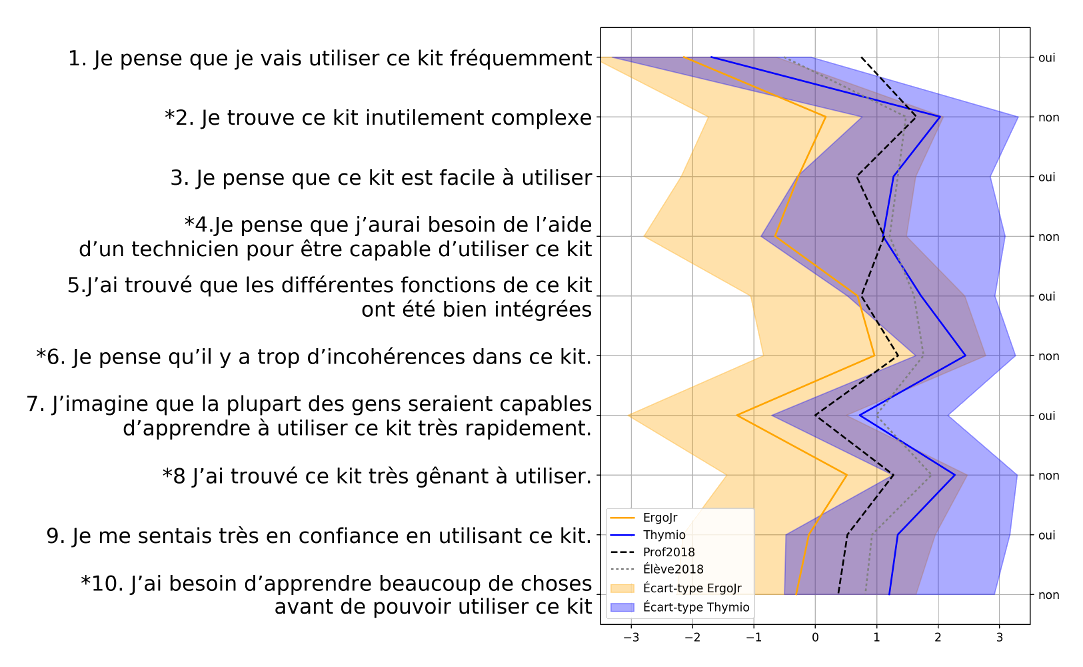
\includegraphics[width=0.9\linewidth]{Figures/Desprez_eiah-sus.png}
                    \caption{Résultats SUS ErgoJr et Thymio~\citeB{desprez:hal-02120958}}\label{fig:sus_vs_thymio}
                \end{figure}\par%
                \begin{figure}[!h]
                    \centering
                    \label{fig:att_vs_thymio}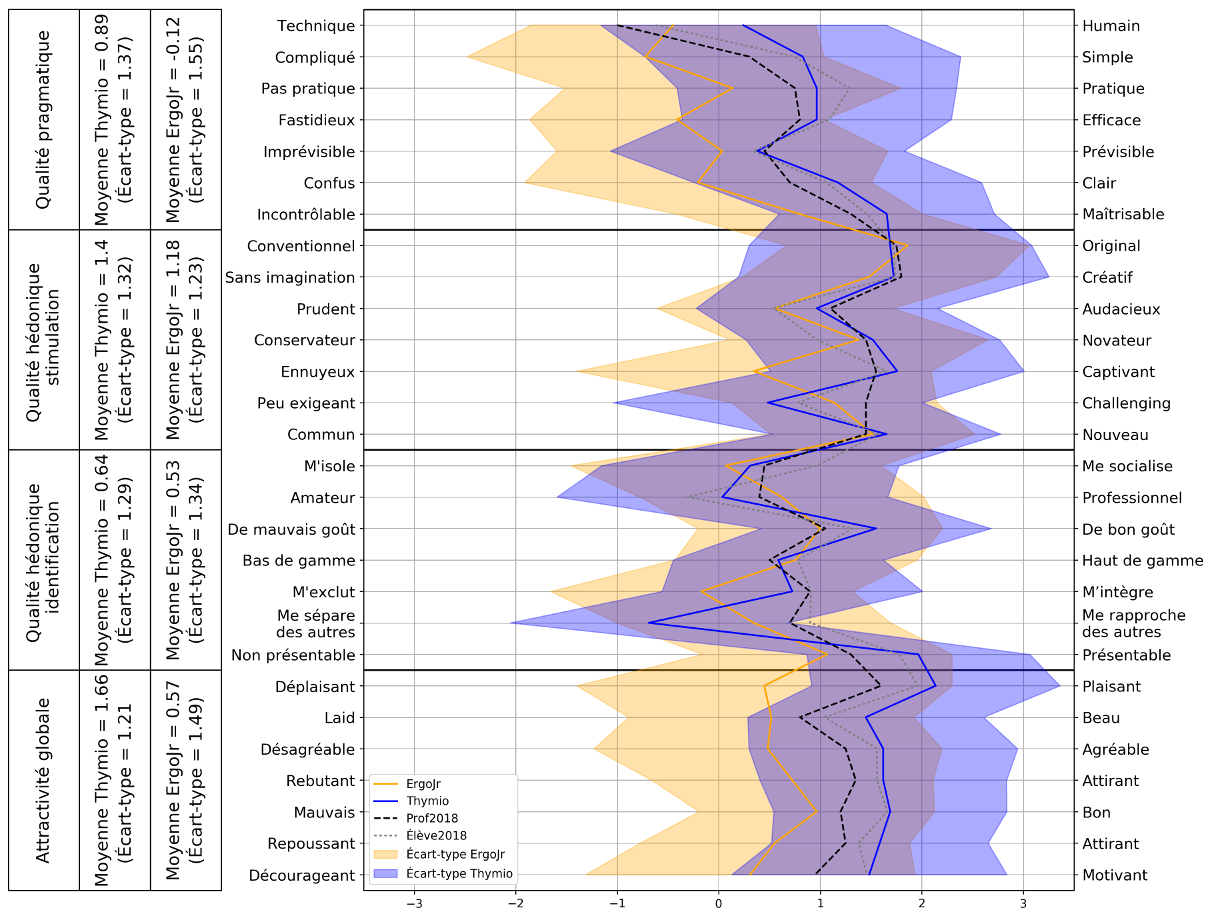
\includegraphics[width=0.9\linewidth]{Figures/Desprez_eiah-atrakdiff.png}
                    \caption{Résultats \textit{AttrakDiff} ErgoJr et Thymio~\citeB{desprez:hal-02120958}}
                \end{figure}\par%
                Le constat est sensiblement identique à celui du SUS: Les résultats sont significativement meilleurs pour le Thymio face au Poppy ErgoJr dans ce contexte de formation ($p=8.36e-5$) mais pas significativement face aux résultats de 2017 ($p=0.34$).
                De plus, nous constatons que c'est principalement sur la 1\iere~et la 4\ieme~échelle qu'est portée cette différence,  et que d'un point de vue uniquement hédonique, aucune plateforme ne se distingue.
    \subsection{Synthèse}
        Ces deux questionnaires \tiret{standardisés} nous ont permis, d'une part de rassembler un certain nombre d'éléments quantifiables afin de mieux évaluer les choix et stratégies de conception pris pour le dispositif Poppy Éducation et ce, principalement sur le kit ErgoJr.
        Cela nous permet de mieux appréhender la pertinence des solutions proposées en fonction des différents usages et perceptions qu'ont les utilisateurs.
        D'autre part, utiliser ces questionnaires nous permet de proposer une \gui{photographie} des caractéristiques d'utilisabilité perçues par l'utilisateur selon différents critères.
        Ceci offre la possibilité de comparaisons futures avec d'autres dispositifs de robotique pédagogique, permettant de mieux classifier ces outils.
        Mais déjà, nous constatons que tant sur l'utilisabilité que sur l'expérience utilisateur, relevées respectivement par le \sht{SUS} et l' \sht{ATT}, nous observons de meilleurs résultats pour le Thymio dans un contexte de formation courte chez un public novice. Cependant, placé dans le contexte pour lequel il a été conçu, c'est à dire, de façon répétée en classe par un public d'élèves et d'enseignants ayant déjà exploré les rudiments de la programmation, le Poppy ErgoJr a obtenu des résultats comparables à celui du Thymio. De plus, au niveau de l'expérience utilisateur les caractéristiques hédoniques des deux plateformes obtiennent des scores similaires, indépendamment du contexte. Ainsi, ces résultats tendent à montrer que le Thymio est plus adapté à l'initiation d'un public novice, là où le Poppy~ErgoJr serait plus adapté à l'approfondissement, et que tous deux sont des plateformes robustes en terme d'utilisabilité.